\documentclass[10pt]{beamer}
\usepackage[spanish]{babel}
\unaccentedoperators
\usepackage[utf8]{inputenc}
\usetheme{Luebeck}
\usepackage{graphicx}

%%%%%%%%%%%%%%%%%%%%%%%%%%%%%%%%%%%%%%%%%%%%%%%%%%%

\title[Función de distribución hipergeométrica]{Función de distribución hipergeométrica}
\author[Adriana Calvo  Misael Peraza  Carolina Yanes]{Adriana Calvo - Misael Peraza - Carolina Yanes \\  Facultad de Matemáticas\\  Universidad de La Laguna}
\date[\today]{\today}

\usetheme{Luebeck}

\definecolor{Mivioleta}{RGB}{122,59,122}
\definecolor{Miazul}{RGB}{0,88,147}
\definecolor{Migris}{RGB}{56,61,66}
\setbeamercolor{palette primary}{use=structure,lg=white,bg=Mivioleta}
\setbeamercolor{palette secundary}{use=structure,lg=white,bg=Miazul}
\setbeamercolor{palette terciary}{use=structure,lg=white,bg=Migris}
\beamertemplateshadingbackground{Mivioleta!88!white}{Miazul!40!white}

%%%%%%%%%%%%%%%%%%%%%%%%%%%%%%%%%%%%%%%%%%%%%%%%%%%%%
\begin{document}
\begin{frame}
\titlepage
\end{frame}

%%%%%%%%%%%%%%%%%%%%%%%%%%%%%%%%%%%%%%%%%%%%%%%%%%%%%%

\begin{frame}
\frametitle{Indice}
\tableofcontents[pausesection]
\end{frame}

%%%%%%%%%%%%%%%%%%%%%%%%%%%%%%%%%%%%%%%%%%%%%%%%%%%%%%%%%

\section{Motivación y objetivos}
\begin{frame}
\frametitle{Motivación y objetivos}

El objetivo principal de este proyecto consiste en aprender a manejar un lenguaje de programación denominado Python, además de usarlo como una herramienta básica en el ámbito matemático. En este trabajo también se encuentran otros objetivos como el de familiarizarse con $\LaTeX$ y Beamer, herramientas básicas en la redacción y exposición de informes y proyectos.

\end{frame}


%%%%%%%%%%%%%%%%%%%%%%%%%%%%%%%%%%%%%%%%%%%%%%%%%%%%%%%%%%%%%

\section{Variable aleatoria Hipergeométrica}
\begin{frame}
\frametitle{Variable aleatoria Hipergeométrica}
\begin{block}{Definición}

Dados $N$, $A$ y $B$  números naturales, se llama {\textbf{variable aleatoria hipergeométrica}} de parámetros ($n$ ,$A$ ,$B$) a una variable que trata de medir el número de ''éxitos'' cuando se extrae una muestra de tamaño $n$ sin reemplazamiento. Su función de probabilidad es:\\

\centerline{$P[\xi = k] = \frac {\binom {A} {k} \binom {B} {n-k}} { \binom {N} {n} }$}
\ \\
$\forall k=0,1,…,n$ y se denota por $\xi \sim H(n ,A ,B)$. Se tiene que:\\
\ \\
$E[\xi] = n \cdot \frac{A}{N}$\\
\ \\
$V(\xi) = n \cdot \frac{A}{N} \cdot \frac{B}{N} \cdot \frac{N-n}{N-1}$\\ 

\end{block}
\end{frame}

%%%%%%%%%%%%%%%%%%%%%%%%%%%%%%%%%%%%%%%%%%%%%%%%%%%%%%%%%%%%%

\section{Procedimiento experimental}
\begin{frame}
\frametitle{Procedimiento experimental}

Aplicándola a dos ejemplos en particular:

De una baraja española de 40 cartas se extraen 5 al azar. Calcúlese la probabilidad de obtener:

\end{frame}

%%%%%%%%%%%%%%%%%%%%%%%%%%%%%%%%%%%%%%%%%%%%%%%%%%%%%%%%%%%%%%%

\subsection{Poker de Ases}
\begin{frame}
\frametitle{Poker de Ases}
\begin{block}{Resultado:}

Para el poker de ases, se tiene que:

\centerline{$P(\xi=x)=\frac {\binom {N_1} {x} \binom {N_2} {n-x}} { \binom {N} {n} }$}

que, en este caso, se traduce en:
\ \\

\centerline{$P(\xi=4)=\frac {\binom {4} {4} \binom {36} {1}} { \binom {40} {5} }=0,000055$}
\ \\

\end{block}
\end{frame}

%%%%%%%%%%%%%%%%%%%%%%%%%%%%%%%%%%%%%%%%%%%%%%%%%%%%%%%%%%%%%%%%

\subsection{Color}
\begin{frame}
\frametitle{Color}
\begin{block}{Resultado:}

Para el color la probabilidad de sacarlo de un determinado palo será:
\ \\

\centerline{$P(\xi=5)=\frac {\binom {10} {5} \binom {30} {0}} { \binom {40} {5} } = 0.000383$} 

\ \\

donde $\xi$ es la variable (número de cartas extraídas de un determinado palo).\\
Pero como la baraja tiene cuatro palos, la probabilidad de obtener color será: \\

\centerline{$P(color)=4\cdot 0,000383=0,001532.$}

\end{block}
\end{frame}

%%%%%%%%%%%%%%%%%%%%%%%%%%%%%%%%%%%%%%%%%%%%%%%%%%%%%%%%%%%%%%%

\section{Algoritmo de la función Hipergeométrica}
\begin{frame}
\frametitle{Algoritmo de la función Hipergeométrica}

{\tiny import math 

import time 

start1 = time.time() 


def fact(p):

\hspace{4mm} a=1
    
\hspace{4mm} if p $<$ 0:
        
\hspace{7mm} return 0
    
\hspace{4mm} elif p==0:
        
\hspace{7mm} return 1
    
\hspace{4mm} else:
        
\hspace{7mm} for i in range(2,p+1):
            
\hspace{10mm} a=a*i
    
\hspace{4mm} return (a)


finish1 = time.time() - start1     
        
A=int(raw\_input('' Introduzca el A (A $>$ x): "))

B=int(raw\_input('' Introduzca el B (B $>$ n-x): "))

n=int(raw\_input('' Introduzca el n: (n $<$ A+B)"))

x=int(raw\_input('' Introduzca la x: "))


N=A+B


start2 = time.time()

comb1=float(fact(A)/(fact(x)*fact(A-x)))

comb2=float(fact(B)/(fact(n-x)*fact(B-n+x)))

comb3=float(fact(N)/(fact(n)*fact(N-n)))

probabilidad=(comb1*comb2)/comb3

print"La probabilidad es :",probabilidad

finish2 = time.time() - start2

finish = finish1 + finish2

print finish}

\end{frame}

%%%%%%%%%%%%%%%%%%%%%%%%%%%%%%%%%%%%%%%%%%%%%%%%%%%%%%%%%%%%%%%%%%%%%

\section{Interpretación Gráfica}
\begin{frame}
\frametitle{Interpretación Gráfica}

A continuación, estudiaremos las probabilidades y tiempo mediante una gráfica de otra muestra dando valores enteros $(A=40, B=10, n=5 ,x=1,...,n).$

\end{frame}

%%%%%%%%%%%%%%%%%%%%%%%%%%%%%%%%%%%%%%%%%%%%%%%%%%%%%%%%%%%%%%%%%%%%%%%

\subsection{Interpretación Gráfica de las probabilidades}
\begin{frame}
\frametitle{Interpretación Gráfica de las probabilidades}
\begin{figure}[!ht]{PROBABILIDADES\\}
\centering
\includegraphics[width=1.1\textwidth]{grafica1.eps}
\caption{Probabilidades}
\end{figure}
\end{frame}

%%%%%%%%%%%%%%%%%%%%%%%%%%%%%%%%%%%%%%%%%%%%%%%%%%%%%%%%%%%%%%%%%%%%%%%

\subsection{Interpretación Gráfica del tiempo}
\begin{frame}
\frametitle{Interpretación Gráfica del tiempo}


\begin{figure}[!ht]{TIEMPO\\}
\centering
\includegraphics[width=1.1\textwidth]{grafica2.eps}
\caption{tiempo}
\end{figure}

\end{frame}

%%%%%%%%%%%%%%%%%%%%%%%%%%%%%%%%%%%%%%%%%%%%%%%%%%%%%%%%%%%%%%%%%%%%%%%

\section{Conclusión}
\begin{frame}
\frametitle{Conclusión}

Esta exposición resume brevemente en lo que ha consistido el proyecto. En él, se ha identificado los propósitos del mismo.
Se ha recopilado información sobre la función de distribución hipergeométrica y se ha implementado este aspecto matemático en el lenguaje de programación de esta asignatura, es decir,el Python.
Por último, se ha adquirido más destreza en el uso de programas como \LaTeX{}~ y Beamer para la creación de textos científicos.

\end{frame}

%%%%%%%%%%%%%%%%%%%%%%%%%%%%%%%%%%%%%%%%%%%%%%%%%%%%%%%%%%%%%%%%%%%%%%%

\section{Bibliografía}
\begin{frame}
\frametitle{Bibliografía}
\begin{thebibliography}{10}
\beamertemplatebookbibitems
\bibitem{}
Francisco Javier Martín-Pliego, José María Montero Lorezno,Luis Ruiz-Maya Pérez. Problemas de Probabilidad 
\bibitem{}
Guido Rossum. Python reference manual. Technical report, Amsterdam, The Netherlands, 1995.
\bibitem{}
Juan José Salazar y Marta López Yurda. Ejercicios Resueltos de probabilidad.

\end{thebibliography}
\end{frame}



\end{document}